% Uncomment this line for on-screen presentation
\documentclass[xcolor={dvipsnames}]{beamer}\usepackage{etoolbox}\newtoggle{printable}\togglefalse{printable}

% Uncomment this line for printable slides (disable animations and don't waste ink)
%\documentclass[handout, xcolor={dvipsnames}]{beamer}\usepackage{etoolbox}\newtoggle{printable}\toggletrue{printable}

% Adjust these for the path of the theme and its graphics, relative to this file
%\usepackage{beamerthemeFalmouthGamesAcademy}
\usepackage{../../beamerthemeFalmouthGamesAcademy}
\graphicspath{ {../../} }

% Default language for code listings
\lstset{language=C++,
		morekeywords={each,in}
}

\begin{document}
\title{IP Law \& Open-Source Licensing}   
\subtitle{COMP140: Creative Computing Hacking}

\frame{\titlepage} 

\begin{frame}{Lecture Objectives}
	Today's lecture will introduce the basics of intellectual property law, focusing on:
	
	\vspace{2ex}
	
	\begin{columns}[onlytextwidth]
		\begin{column}{0.5\textwidth}
			\begin{itemize}
				\item Ownership \& Contracts
				\item Copyright
				\item Moral Rights
				\item Trademark
			\end{itemize}
		\end{column}
		\begin{column}{0.5\textwidth}
			\begin{itemize}
				\item Design Rights
				\item Trade Secrets
				\item Patents
				\item Licences
			\end{itemize}
		\end{column}
	\end{columns}
	
	\vspace{3ex}
	
	The information in this workshop is for educational purposes only. It is not being delivered
	by a legal expert and its content does not constitute legal advice.
	
\end{frame}

\begin{frame}{Lecture Objectives}
	Today's lecture will also go into more depth with respect to open-source licences, focusing on:
	
	\vspace{2ex}
	
	\begin{itemize}
		\item Creative Commons Licences
		\item MIT Licence
		\item Apache Licence
		\item GNU General Public Licence
	\end{itemize}
	
	\vspace{2ex}
	
	The information in this workshop is for educational purposes only. It is not being delivered
	by a legal expert and its content does not constitute legal advice.
\end{frame}

\begin{frame}{Further Reading}
	\begin{itemize}
		\item Ibrahim, M. (2009) `Legal Issues in Game Development'. In: Sikora, D. and Hattan, J. (Eds.) \textit{Business and Production for Games: A GameDev.net Collection}.
		Cengage Learning: New York.
		\vspace{2ex}
		\item Ibrahim, M. (2009) `Analysis: Clone Games and Fan Games --- Legal Issues'. In: \textit{Gamasutra}
		\url{http://www.gamasutra.com/view/news/117234/Analysis_Clone_Games__Fan_Games__Legal_Issues.php}.
	\end{itemize}
\end{frame}

\begin{frame}{Further Reading}
	\begin{itemize}
		\item Brathwaite, B. and Schreiber, I. (2009) \textit{Challenges for Game Designers: Non-Digital Exercises for Video Game Designers}. Charles
		River Media: Boston, MA.
		\vspace{2ex}
		\item Stein, J. (2015) \textit{The Legal Nature of Video Games --- Adapting Copyright Law to Multimedia}. Press Start, vol. 2, no. 1, pp. 1---13.
		\vspace{2ex}
		\item Stein, J. (2015) \textit{Authorship and Moral Rights in Video Games}. Press Start, vol. 2, no. 2, pp. 1---13.
	\end{itemize}
\end{frame}

\begin{frame}{Further Reading}
	\begin{itemize}
		\item Samuelson, P., Denber, M., and Glushko, R.J. (1992) \textit{Developments on the Intellectual Property Front}. Communications of the ACM, vol. 35, no. 6, pp. 33---39.
		\item Samuelson, P. (2008) \textit{Hacking Intellectual Property Law}. Communications of the ACM, vol. 51, no. 1, pp. 65---67.
		\item Samuelson, P. (2015) \textit{Software Patents Are Falling Down}. Communications of the ACM, vol. 58, no. 11, pp. 27---29.
	\end{itemize}
\end{frame}

\begin{frame}{Further Reading}
	\begin{itemize}
		\item Robert W. Gomulkiewicz, De-bugging Open Source Software Licensing, 64 U. Pitt. L. Rev. 75 (2002)
		\vspace{2ex}
		\item Robert W. Gomulkiewicz, How Copyleft Uses License Rights to Succeed in the Open Source Software Revolution and the Implications for Article 2B, 36 Hous. L. Rev. 179 (1999)
	\end{itemize}
\end{frame}

\begin{frame}{Important Notice}
	This is the final week prior to the Easter break. The University will be closed on Good Friday.
\end{frame}

\part{Intellectual Property}
\frame{\partpage}

\begin{frame}{Learning Outcomes}
	In this section you will learn how to...
	
	\begin{itemize}
		\item \textbf{Distinguish} between the structure of civil law \textbf{and} criminal law
		\item \textbf{Explain} the importance of ownership issues and contracts in game development
		\item \textbf{Explain} what copyright, moral rights, trademarks, design rights, trade secrets, and patents are.
		\item \textbf{Discuss} the role of licensing in intellectual property usage and management
	\end{itemize}
\end{frame}

\begin{frame}{Civil vs Criminal Law}
	\begin{itemize}
		\item \textbf{criminal law}: the body of law dealing with crimes and their punishment. Law sets out all the things which are considered 
		unacceptable, and which will render someone liable for prosecution.
		\vspace{2ex}
		\item \textbf{civil law}: the body of law dealing with disputes between individuals, organisations, and other bodies. It is a very 
		complicated system which tries to set out rules to cover all the sorts of situation that may arise in life, and provides for disputes 
		to be decided by a Judge if the parties are unable to sort it out themselves.
	\end{itemize}
\end{frame}

\begin{frame}{Civil vs Criminal Law}
	\begin{itemize}
		\item Businesses can engage in criminal acts. Such acts include: fraud, industrial espionage, and tax evasion.
		\vspace{2ex}
		\item Most acts, however, are civil in nature. Such acts include: failure to pay bills; breaches of contract; and misuse of intellectual property.
	\end{itemize}
\end{frame}

\begin{frame}{Civil vs Criminal Law}
The reasons why is because UK law has many different sources, some of which include:

	\begin{itemize}
		\item \textbf{statute}: legislation from UK Parliaments and its devolved counterparts.
		\vspace{1ex}
		\item \textbf{`common law'}: principles established through historic cases.
		\vspace{1ex}
		\item \textbf{EU}: regulations and directives set by Europe for all EU citizens.
	\end{itemize}
\end{frame}

\begin{frame}{Civil vs Criminal Law}
	\begin{itemize}
		\item An interesting characteristic of the law in England is the `doctrine of judicial precedents': the judgements of the 
		courts are a binding source of law for future cases. 
		\vspace{1ex}
		\item Judges are bound by the judgements of courts of a higher jurisdiction (although not those of the lower courts).
		\vspace{1ex}
		\item Often appeals processes are based on making a distinction from such historic cases or on the basis of lower courts misinterpreting the law.
	\end{itemize}
\end{frame}

\begin{frame}{Civil vs Criminal Law}
	\begin{itemize}
		\item In civil courts, the claimant assembles their case, with the standard of proof being the ‘balance of probabilities’: the case must be more likely
		to be correct than incorrect.
		\vspace{2ex}
		\item In criminal courts, the prosecution have the burden of proof, and the standard is much higher: they have to prove their 
		case `beyond reasonable doubt'.
	\end{itemize}
\end{frame}

\begin{frame}{Intellectual Property}
	\begin{itemize}
		\item IP law is designed to reward and motivate the contributions of human intellect.
		\item This is achieved by granting certain rights which are commercially valuable.
		\item Essentially, the right to make profit from the actualisation and application of your ideas.
	\end{itemize}
\end{frame}

\begin{frame}{Intellectual Property}
	\begin{itemize}
		\item IP law is covered by the civil courts.
		\item Do not breach IP law, as you may be sued.
		\item Even if, you are not making money yourself, you may be denying profit to the defendant. 
		Even if you are not worth suing because you have no money, they may remedy the situation with
		 injunctions and take-down notices.
		\item IP owners have a legal responsibility to actively protect their works, or risk losing their rights.
	\end{itemize}
\end{frame}

\begin{frame}[fragile]{Socrative \texttt{JBYPC3BBY}}
\textit{Alice is a computer programmer. In her free time, she programs a game. Alice, however, is not an artist.
She asks Brian, a friend, for help. Brian agrees and contributes artwork to the game. No compensation is discussed
and no written agreement exists.}
\vspace{2ex}
	\begin{itemize}
		\item \textbf{Who} owns the game overall? 
		\item In pairs, discuss who owns the game overall for 2 minutes.
		\item\textbf{Select} your choice.
	\end{itemize}
\end{frame}

\begin{frame}{Ownership \& Contracts}
	\begin{itemize}
		\item When more than one person contributes to a work and no agreement exists, co-authors are joint owners
		and everyone retains an equal share in the entire work (Ibrahim, 2009).
		\item In an employer/employee context, the employer always owns the copyright (Ibrahim, 2009). This is implicit
		within your contract of employment.
		\item In a client/worker context, an intellectual property transaction is set out as a contract. Typically, the IP belongs
		to the creator of a work, but in the case of contract work it will likely be transferred to another party as part of the contract.
	\end{itemize}
\end{frame}

\begin{frame}{Ownership \& Contracts}
Contracts require several things to be valid (Ibrahim, 2009):

	\begin{itemize}
		\item Capacity
		\item Mutual Assent
		\item Legal Purpose
		\item Bargained-for Consideration
		\item A Signed-Writing*
	\end{itemize}
\end{frame}

\begin{frame}{Copyright}
	\begin{itemize}
		\item Copyright protects a work from being: translated, copied, publicly performed/transmitted/broadcast, and adapted.
		\item Any time someone copies, performs, or displays a copyrighted work without
		permission, they commit copyright infringement.
		\item Specifically, it protects only expressions, and not ideas.
		\item Copyright has a limited duration, after which work goes into the public domain.
	\end{itemize}
\end{frame}

\begin{frame}{Copyright}
`Fair dealing' exceptions exist:

	\begin{itemize}
		\item Non-commercial research
		\item Private study
		\item Criticism, Review, and Reporting
		\item Teaching
		\item Assistance for Disabled People
		\item Time-shifting
		\item Parody
		\item Orphan Works
	\end{itemize}
\end{frame}

\begin{frame}{Moral Rights}
	\begin{itemize}
		\item Protect the personal interests of the author of a copyrighted work.
		\item Moral rights include:
		\begin{itemize}
			\item Right to be identified
			\item Right to object to derogatory treatment
			\item Right to object to false attribution
			\item Right to privacy
		\end{itemize}
	\end{itemize}
\end{frame}

\begin{frame}{Trademark}
	\begin{itemize}
		\item Trademarks identify the source and/or quality of a product or service.
		\item Protects branding and brand names, so long as its use does not become diluted.
		\item Registration of a trademark is advised as it strengthens its validity, but 
		protection is automatic once brand names are used in commercial transactions.
		\item Most registered trademarks are internationally-binding through the Madrid Protocol.
	\end{itemize}
\end{frame}

\begin{frame}{Design Rights}
	\begin{itemize}
		\item Protects the (3D) shape of a product. Enables a design to be distinctive.
		\item Often used to protect particular user interface elements which are novel.
		\item Does not extend to other aesthetic properties.
		\item Right applies to UK/EU inventors.
	\end{itemize}
\end{frame}

\begin{frame}{Trade Secrets}
	\begin{itemize}
		\item Trade secrets are secrets that have commercial value.
		\item For a valid trade secret to exist, the company claiming a trade secret must
		clearly determine what it is and will take steps to keep it concealed.
		\item Often, takes the form of Non-Disclosure Agreements (NDAs).
		\item Breach of an NDA can result in substantial damages being awarded.
	\end{itemize}
\end{frame}

\begin{frame}{Patents}
	\begin{itemize}
		\item Protects inventions, processes, methods, and products
		\item Criteria include: novel, inventive (not obvious to a skilled person), and capable of industrial application.
		\item Must be registered formally and examined.
		\item Difficult and expensive to obtain, but provides a monopoly over the invention for a period of time.
		\item In exchange for public disclosure, protects the idea behind the invention.
		\item Patents can be territorial or international via the Paris Convention.
	\end{itemize}
\end{frame}

\begin{frame}{Licenses}
	\begin{itemize}
		\item A licensing agreement is a partnership between an intellectual property owner (licensor) and another 
		who is authorized to use such rights (licensee) in exchange for an agreed payment, be that a fee or a royalty.
		\item Includes: technology license; end-user license; trademark franchising agreement; copyright license agreement; etc.
		\item Licensing can broaden the reach of IP into different markets, without the holder incurring risks.
		\item Sometimes there are databases endorsing a `license of right' which means the IP holder grants permission
		to anyone who asks, usually for a fee or a set royalty agreement.
	\end{itemize}
\end{frame}

\part{Practical Activity}
\frame{\partpage}

\begin{frame}[fragile]{Socrative \texttt{JBYPC3BBY}}
	\begin{itemize}
		\item \textbf{Self-organise} into your COMP150 groups.
		\item \textbf{Select} a well-known intellectual property: Mass Effect; Star Craft; Mario; Crazy Taxi.
		\item \textbf{Discuss} on Slack for 15 minutes the legal implications of using any of their IP.
		\vspace{2ex}
		\item \textbf{Summarise FIVE} key IP laws that prevent you from using elements from the IP.
	\end{itemize}
\end{frame}

\part{Open Source Software Licenses}
\frame{\partpage}

\begin{frame}{Learning Outcomes}
	In this section you will learn how to...
	
	\begin{itemize}
		\item \textbf{Recognise} the philosophy of open-source licensing and its benefits
		\item \textbf{Differentiate} between the Creative Commons, MIT, Apache, and GNU General Public Licenses
		\item \textbf{Suggest} the most appropriate license for a given circumstance
	\end{itemize}
	
	This section has been adapted from the talk `A Lawyer Looks at the Open Source Revolution' by Robert W. Gomulkiewicz.
\end{frame}

\begin{frame}{Open Source}
	\begin{itemize}
		\item Source = software in source code form
		\item Open = freedom to:
		\begin{itemize}
			\item View the source code
			\item Run the software for any purpose
			\item Modify the software in any way
			\item Distribute the software and any modifications
		\end{itemize}
		\item Software Development Model
		\item Philosophy --- Share and Collaborate
		\item Licensing Model
	\end{itemize}
\end{frame}

\begin{frame}{Open Source}
	\begin{itemize}
		\item Opposite of `proprietary' (`commercial') software:
		\begin{itemize}
			\item Hold the source code as a trade secret
			\item Distribute software as a binary
			\item Limited licensing for derivative works
			\item Buggy, and difficult to extend
		\end{itemize}
	\end{itemize}
\end{frame}

\begin{frame}{Open Source}
Notable names in Open Source:

	\begin{itemize}
		\item Richard Stallman (Free Software Foundation)
		\item Eric Raymond (The Cathedral and the Bazaar)
		\item Linus Torvalds (Linux)
		\item Bruce Perens (Open Source Definition)
	\end{itemize}
\end{frame}

\begin{frame}{Open Source}
\textit{``Given enough eyeballs, all bugs are shallow''}
--- Eric Raymond
\end{frame}

\begin{frame}{Open Source}
Advantages of open-source:

	\begin{itemize}
		\item Scratching an itch to fix or extend something
		\item Forking and Pull-Requests
		\item Peer Review
		\item Centralized decision-making
	\end{itemize}
\end{frame}

\begin{frame}{Open Source}
	\begin{itemize}
		\item Software has always traditionally been shared by scientists and hobbyists
		\item The Internet and WWW makes sharing and collaboration very efficient
		\item Watershed: Netscape licensed Communicator under an open source license
		\item Linux+Apache became the most popular web server
		\item Ever-increasing adoption
	\end{itemize}
\end{frame}

\begin{frame}{Open Source}
As a business model:

	\begin{itemize}
		\item ``Think `free speech', not `free beer''' --- Richard Stallman
		\item Branded distributions
		\item Sell hardware, give away software
		\item Sell services and support
		\item Dual versions, dual licensing
		\item Value added software
		\item Sell sponsorships, ads, and T-shirts
	\end{itemize}
\end{frame}

\begin{frame}{Open Source}
Free and open is not:

	\begin{itemize}
		\item Public domain
		\item Copyright `first sale'
		\item Shareware or freeware
	\end{itemize}
\end{frame}

\begin{frame}{Open Source}
Licenses (and IP law) make it work:

	\begin{itemize}
		\item Control and limitations over use
		\item Risk shifting
		\item To remain free (and worthwhile), software must be copyrighted and licensed
	\end{itemize}
\end{frame}

\begin{frame}{Creative Commons}
Key terms:

	\begin{itemize}
		\item Flexible. Can be customised.
		\item BY = Attribution.
		\item SA = Share Alike.
		\item ND = No Derivatives.
		\item NC = Non-Commercial.
	\end{itemize}
\end{frame}

\begin{frame}{BSD Licence}
	\begin{itemize}
		\item License grant:  unlimited use, modification, distribution
		\item No warranties; disclaimer of consequential damages
		\item No endorsement
		\item Attribution required.
	\end{itemize}
\end{frame}

\begin{frame}{MIT Licence}
	\begin{itemize}
		\item commercial use
		\item can modify
		\item can distribute
		\item can sub-license
		\item private use
		\item cannot hold liable
		\item must include copyright notice
		\item must include copy of license in distribution
	\end{itemize}
\end{frame}

\begin{frame}{Apache Licence}
	\begin{itemize}
		\item freely download and use Apache software, in whole or in part, for personal, company
		 internal, or commercial purposes;
		\item use Apache software in packages or distributions that you create.
		\item must redistribute any piece of Apache-originated software with proper attribution;
		\item must not use any marks owned by The Apache Software Foundation in any way that 
		might state or imply that the Foundation endorses your distribution;
	\end{itemize}
\end{frame}

\begin{frame}{Apache Licence}
	\begin{itemize}
		\item must not use any marks owned by The Apache Software Foundation in any way that
		 might state or imply that you created the Apache software in question.
		\item must include a copy of the license in any redistribution you may make that includes Apache software;
		\item must provide clear attribution to The Apache Software Foundation for any distributions that include Apache software.
	\end{itemize}
\end{frame}

\begin{frame}{GNU General Public Licence}
	\begin{itemize}
		\item Unlimited right to run program
		\item Unlimited access to source code
		\item Unlimited right to distribute verbatim copies
		\item May create derivatives IF you agree to make the derivatives “free”
		\item License is “viral”
		\item No warranties; disclaimer of consequential damages
	\end{itemize}
\end{frame}

\part{Practical Activity}
\frame{\partpage}

\begin{frame}[fragile]{Socrative \texttt{JBYPC3BBY}}
In your teams:
	\begin{itemize}
		
		\item \textbf{Research} the SCO litigation case.
		\item \textbf{Discuss} the litigation for 10 minutes on Slack.
	
		\item \textbf{State ONE} fact about the case for EACH member in your group.
	\end{itemize}
\end{frame}

\begin{frame}[fragile]{Socrative \texttt{JBYPC3BBY}}
In your teams:
	\begin{itemize}
		
		\item \textbf{Research} the licenses in more depth.
		\item \textbf{Discuss} which license is most suited to your COMP150 game for 10 minutes on Slack.
	
		\item \textbf{Suggest ONE} license \textbf{and justify why} you chose it.
	\end{itemize}
\end{frame}

% Move this to next week
%\part{Functions}
\frame{\partpage}

\begin{frame}[fragile]{Function definitions}
    \begin{itemize}
        \item We have already seen an example of a function definition
    \end{itemize}
    \begin{lstlisting}
int main()
{
    std::cout << "Hello, world!" << std::endl;
    return 0;
}
    \end{lstlisting}
    \begin{itemize}
        \item The function \lstinline{main} takes no parameters, and returns a value of type \lstinline{int}
    \end{itemize}
\end{frame}

\begin{frame}[fragile]{Function signatures}
    \begin{itemize}
        \item The \textbf{signature} of a function defines its return type, name, and parameters
    \end{itemize}
    \begin{lstlisting}
double foo(std::string x, int y, bool z)
    \end{lstlisting}
    \pause
    \begin{itemize}
        \item This function takes three parameters: \pause
        \lstinline{x} of type \lstinline{std::string}, \pause
        \lstinline{y} of type \lstinline{int}, \pause
        and \lstinline{z} of type \lstinline{bool} \pause
        \item It returns a value of type \lstinline{double}
    \end{itemize}
\end{frame}

\begin{frame}[fragile]{Functions without return values}
    \begin{itemize}
        \item It is possible to define a function which does not return a value, using the \lstinline{void} keyword
        in place of its return type
    \end{itemize}
    \pause
    \begin{lstlisting}
void printNumber(int n)
{
    std::cout << n << std::endl;
}
    \end{lstlisting}
\end{frame}

\begin{frame}[fragile]{Pass by value}
    \begin{itemize}
        \item Function parameters are passed \textbf{by value}:
        the function receives \textbf{copies} of the original variables
    \end{itemize}
    \pause
    \begin{lstlisting}
void changeName(std::string name)
{
    name = "Ed";
}

int main()
{
    std::string name = "Mike";
    std::cout << name << std::endl; // Mike
    changeName();
    std::cout << name << std::endl; // Mike
}
    \end{lstlisting}
\end{frame}

\begin{frame}[fragile]{Pass by reference}
    \begin{itemize}
        \item Parameters can be passed \textbf{by reference} using \lstinline{&}, allowing the function to modify them
    \end{itemize}
    \pause
    \begin{lstlisting}
void changeName(std::string& name)
{
    name = "Ed";
}

int main()
{
    std::string name = "Mike";
    std::cout << name << std::endl; // Mike
    changeName();
    std::cout << name << std::endl; // Ed
}
    \end{lstlisting}
\end{frame}

\begin{frame}[fragile]{One area where C++ is ``simpler'' than Python!}
    \begin{itemize}
        \item Recall from COMP110 week 6: in Python, basic data types (numbers, booleans, strings etc)
            are passed by value, and object types (lists, dictionaries, class instances) are passed by reference
        \pause
        \item In C++, everything is passed by value unless it is explicitly marked as a reference with \lstinline{&}
    \end{itemize}
\end{frame}

\begin{frame}[fragile]{Constant references}
    \begin{lstlisting}
void greet(std::string name)
{
    std::cout << "Hi " << name << std::endl;
}
    \end{lstlisting}
    \pause
    \begin{itemize}
        \item The string will be copied in order to be passed in \pause
        \item More efficient to pass a reference, and mark it \lstinline{const} to prevent accidental modification
    \end{itemize}
    \begin{lstlisting}
void greet(const std::string& name)
{
    std::cout << "Hi " << name << std::endl;
}
    \end{lstlisting}
    \pause
    \begin{itemize}
        \item (this is only worthwhile for large data structures like strings and vectors, not for basic data types)
    \end{itemize}
\end{frame}



\part{Practical Activity}
\frame{\partpage}

\begin{frame}{API Proposal}
	\begin{itemize}
		\item \textbf{Write} your proposal.
		\item Do this in a Markdown document in the COMP140 GitHub repository.
		\item You have 15 minutes.
	\end{itemize}
\end{frame}
		
\begin{frame}{API Proposal Review}
	\begin{itemize}	
		\item \textbf{Swap} proposals with another student.	
		\item \textbf{Review} the proposal that you have received.
		\item \textbf{Assess} the scope and feasibility of the proposal.
		\item \textbf{Assess} the novelty and potential utility of the proposed plug-in.
		\item \textbf{Assess} the commercial awareness demonstrated in the proposal.
		\item \textbf{Complete} the review form.
		\vspace{2ex}
		\item You have 25 minutes.
	\end{itemize}
\end{frame}

\begin{frame}{Coursework Progress}
You should, by now, have:

	\begin{itemize}
		\item \textbf{Identified} partners for the API task, where appropriate.
		\item \textbf{Developed} a draft proposal. 
	\end{itemize}
	
You should, now:

	\begin{itemize}
		\item \textbf{Revise} the proposal.
		\item \textbf{Make} a pull request by Thursday for tutors to review. 
		\item Once approved, \textbf{commence} prototype development. 
	\end{itemize}
\end{frame}

% -------------------------------------------------------

%\part{The compiler}
%\frame{\partpage}
%
%\begin{frame}
%	\frametitle{The build process}
%	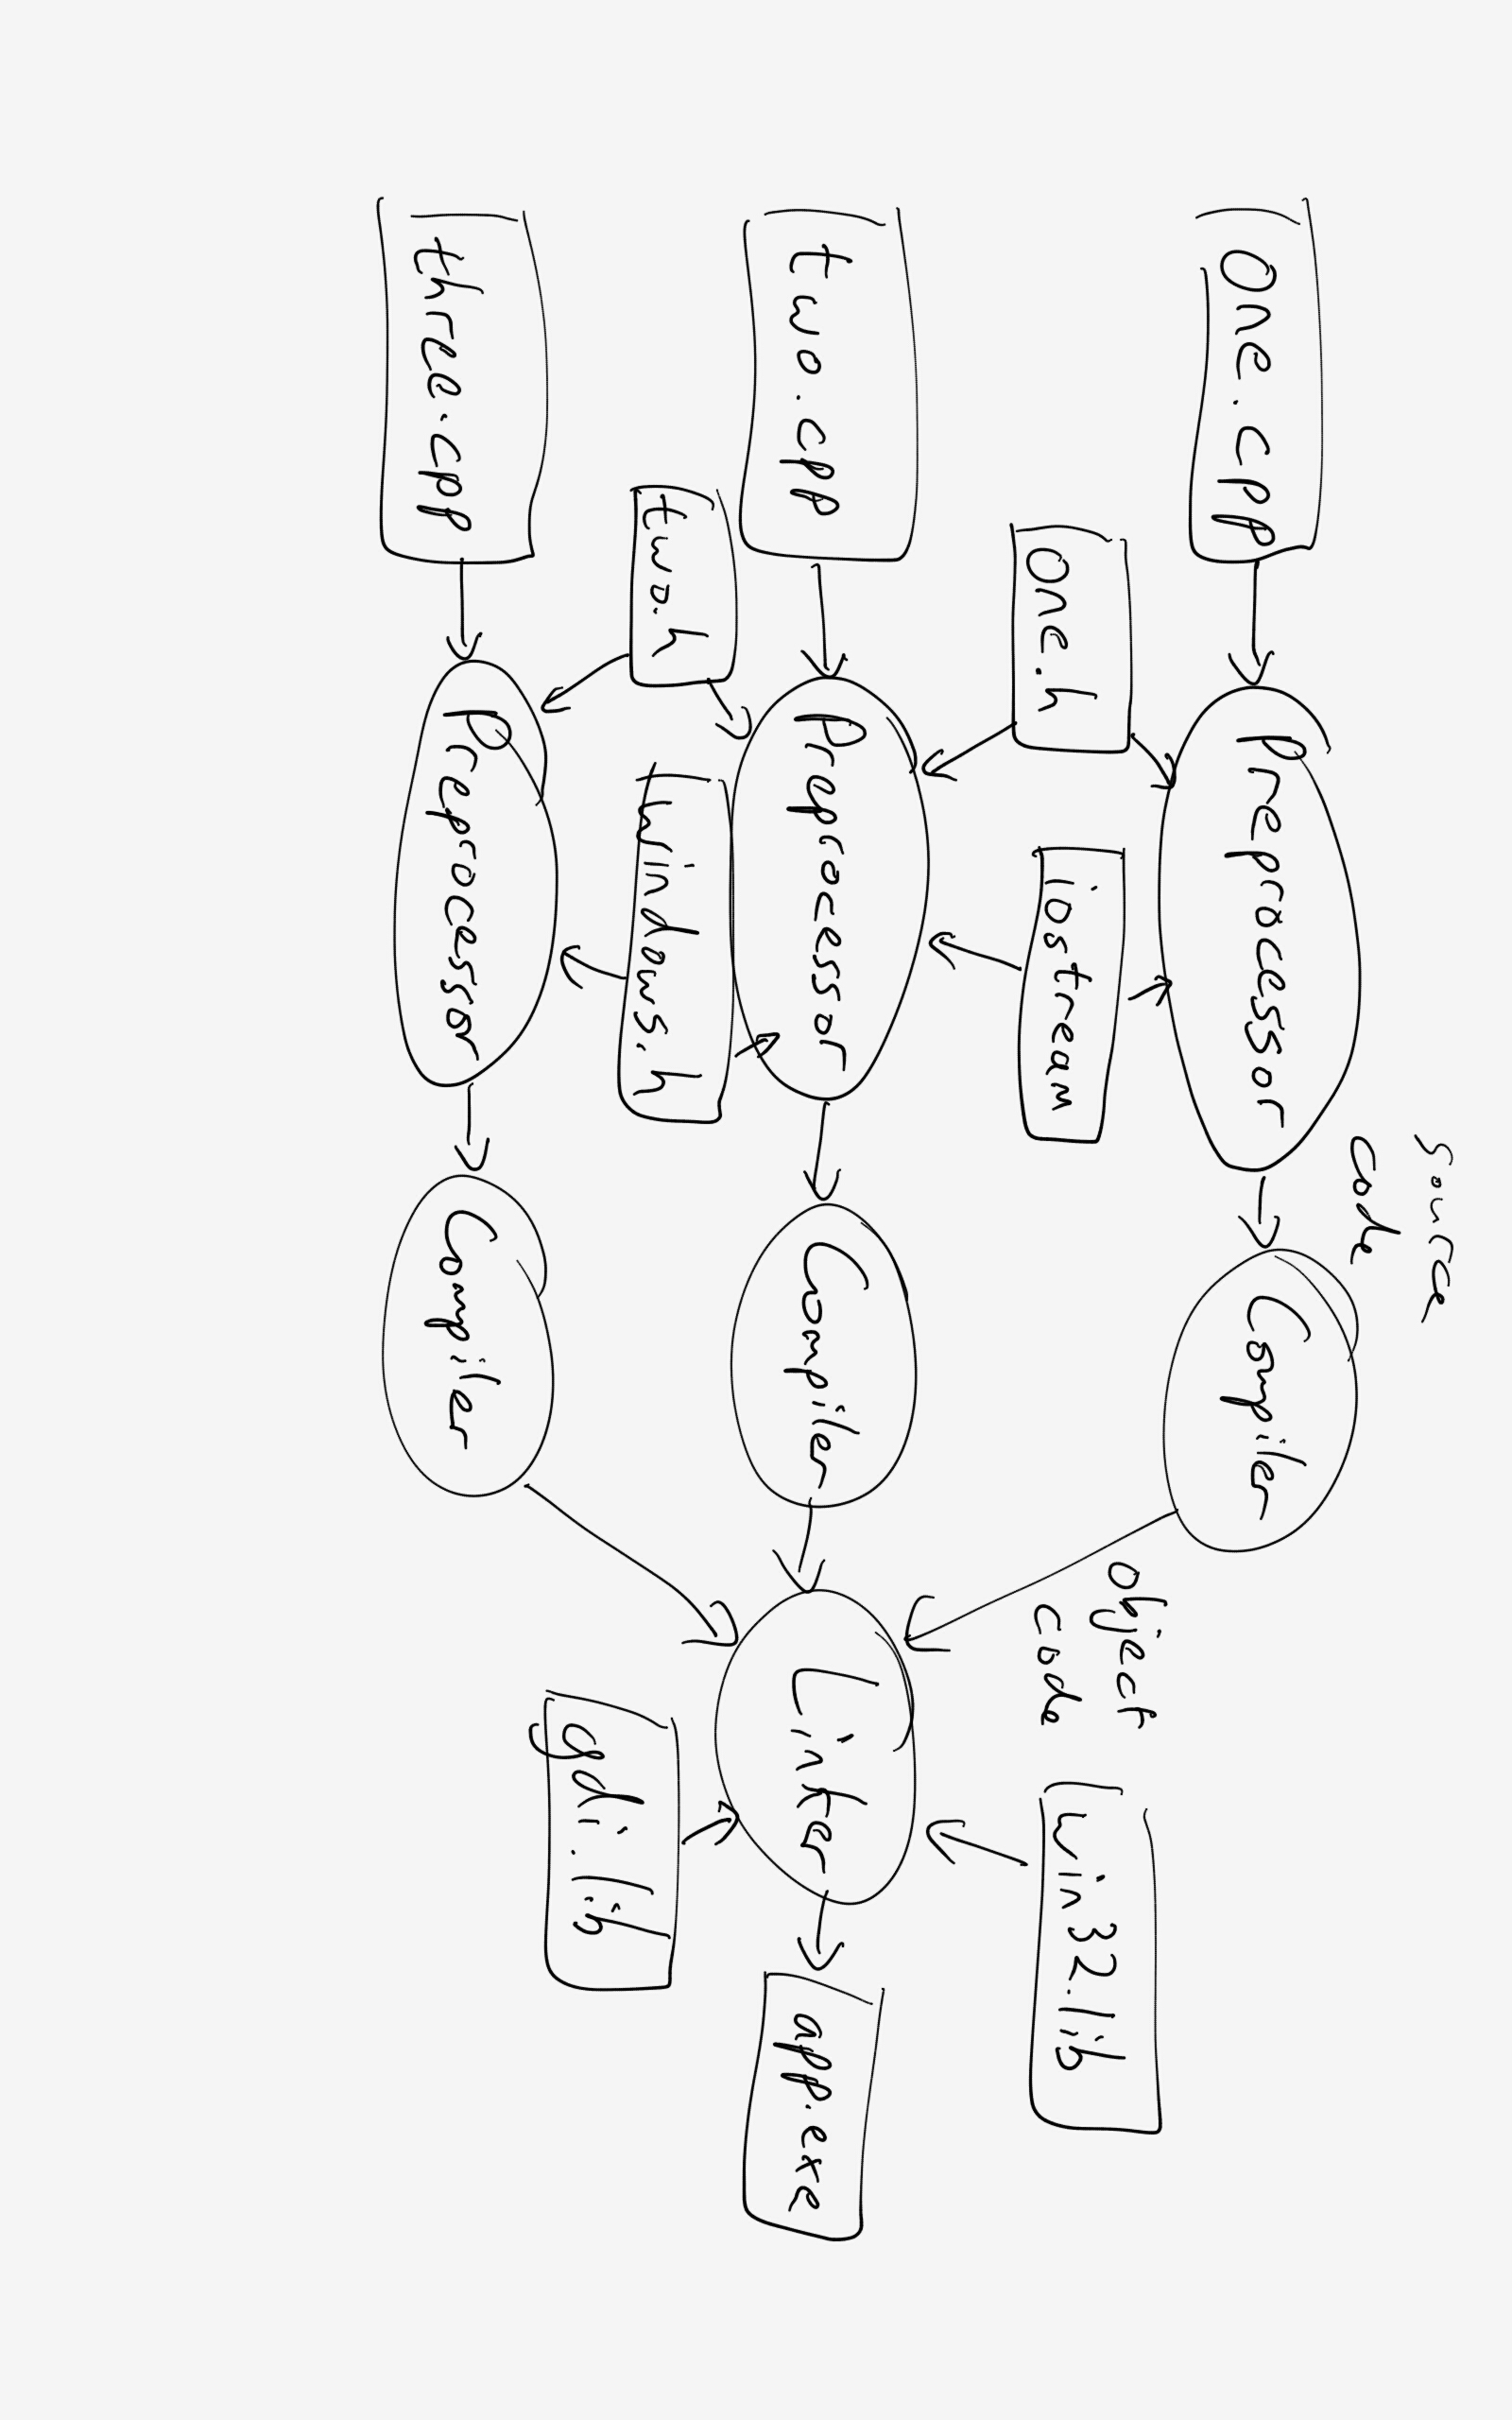
\includegraphics[height=\textwidth,angle=90]{compiler_sketch}
%\end{frame}

\end{document}
